\documentclass[12pt,letterpaper]{article}
\usepackage[utf8]{inputenc}
\usepackage[spanish]{babel}
\renewcommand{\baselinestretch}{1.5} %Interlineado 
\usepackage[left=4cm,top=3cm,right=3cm,bottom=3cm]{geometry} %Definición de los margenes
\clubpenalty=10000 %Penalización_Lineas_huerfanas
\widowpenalty=10000 %Penalización_Lineas_viudas
\usepackage{enumerate} %Para editar formato enumerate
\usepackage{pdfpages} %insertar pdf.
\usepackage{color}
\usepackage{url} %definicion de url
\usepackage[hidelinks]{hyperref} % quitar cajas de hipervinculos

\begin{document}		

\begin{titlepage}	
\begin{center}
\textsc{universidad central de venezuela\\facultad de ingeniería\\escuela de ingeniería eléctrica\\departamento de comunicaciones\\anteproyecto de trabajo de grado\\}
\vspace*{5cm}
IMPLEMENTACIÓN DEL PROTOCOLO H.239 EN UNA UNIDAD DE CONTROL MULTIPUNTO (MCU) BASADO EN CÓDIGO ABIERTO PARA LA COMPARTICION DE DATOS EN FORMATO DUAL STREAM.
\end{center}
\vspace*{4cm}

\begin{flushright}
{\footnotesize Anteproyecto de trabajo de grado a ser\\considerado por el Departamento de\\Comunicaciones para optar al título de\\Ingeniero Electricista.}\\
\vspace*{1cm}Br. Ángel J. Oramas I.\\C.I 18.854.050
\end{flushright}

\vfill \centerline {Caracas, Enero de 2017.}	
\end{titlepage}

\newpage
\centerline{\textbf{TÍTULO}}

Implementación del protocolo H.239 en una Unidad de Control Multipunto (MCU) basado en código abierto para la compartición de datos en formato \emph{dual stream}.

\centerline{\textbf{INTRODUCCIÓN}}

El gran avance que ha tenido el desarrollo de las Tecnologías de la Información y la Comunicación\footnote{TIC. \emph{Tecnologías de la Información y la Comunicación}.} en las últimas décadas, ha permitido que su aplicación en el sector salud sea cada vez frecuente, logrando importantes mejorías en la atención al paciente y en la calidad de los servicios prestados, así como una significativa reducción de los costos  operativos y administrativos.

En Venezuela, el uso de TIC en la salud se remonta a la década de los 90, principalmente a nivel de investigación en diversas entidades académicas y centros universitarios orientados hacia las  áreas de las telecomunicaciones y telemedicina, desarrollo de \emph{software} para registro clínico, procesamiento de imágenes médicas y aplicaciones web.

Uno de los proyectos de gran importancia para la comunidad médica del país es SOS\footnote{SOS. \emph{Segunda Opción en Salud}.} Telemedicina para Venezuela, resultado del esfuerzo y continuo trabajo que data desde 1996 y es liderado por el Centro de Análisis de Imágenes Biomédicas Computarizadas\footnote{CAIBCO. \emph{Centro de Análisis de Imágenes Biomédicas Computarizadas}.} en la Facultad de Medicina de la UCV, con el objetivo fundamental de mejorar la calidad resolutiva del servicio público nacional de salud mediante el diseño, desarrollo, implementación y puesta en marcha de un sistema de telemedicina que conecte en red a centros remotos de atención primaria de salud con especialistas de la Universidad Central de Venezuela y otras universidades nacionales e internacionales; dedicadas a la investigación, a la transferencia de tecnologías, al equipamiento y soporte de la plataforma tecnológica, a la capacitación del personal de la salud, a la evaluación e intercambio de opiniones sobre casos médicos y sus posibles soluciones. 

Es importante señalar, que en más de 10 años de experiencias, con la colaboración de estudiantes de pregado y postgrado, profesores, personal administrativo, profesionales y expertos de diversas facultades y dependencias adscritas a la UCV, el proyecto se ha consolidado satisfactoriamente y en la actualidad se cuenta con una red en expansión, de arquitectura abierta con aplicaciones propias desarrolladas tanto en \emph{software} libre como en \emph{software} propietario de importantes empresas (HP, Cisco, Microsoft, entre otras), empleando diferentes TIC que gestionan grandes bases de datos alojados en servidores, protocolos de comunicación, estándares de interoperabilidad, lenguajes de programación; para ofrecer soluciones tecnológicas de teleconsulta, telediagnóstico y teleducación a través de videoconferencias, acceso a distinto portales web con temáticas sobre la salud, acceso al historial clínico electrónico, entre otras. 

La red y sus tecnologías son impulsadas a través de varias instancias relacionadas al proyecto, siendo una de ellas, el Centro de Informática de Medicina\footnote{CIM. \emph{Centro de Informática de Medicina}.}, donde se encargan de mantener operativos y funcionales los equipos que conforman la plataforma a través de correctas políticas de uso y de seguridad. 
   
\centerline{\textbf{PLANTEAMIENTO DEL PROBLEMA}}


Debido a su labor, es como surge la necesidad de realizar este trabajo, ya que actualmente uno de los equipos de la plataforma, específicamente la Unidad de Control Multipunto\footnote{MCU. \emph{Multipunt Control Unit, por sus siglas en inglés.}}, equipo que forma parte del sistema de videoconferencia se encuentra inhabilitado.

Ante tal situación, el Departamento de Telecomunicaciones del CIM optó por implementar una Unidad de Control Multipunto \emph{software} libre y código abierto, la cual se encuentra alojado en un servidor de la Facultad de Medicina en el Data Center de la UCV; y maneja la mayoría de los protocolos de comunicación para ofrecer servicio de videoconferencia. Sin embargo, es importante mencionar que una de las características que no presenta, es la de incluir en el stack de protocolos al H.239, principalmente responsable en la gestión de compartición de datos sobre vídeo (\emph{dual stream}) en una sesión de videoconferencia, condición que afecta de manera cualitativamente, la calidad del servicio (QoS) \footnote{QoS. \emph{Quality of Service, por sus siglas en inglés.}} que se desea ofrecer.

Por esto es necesario hacer un estudio que permita la adición del protocolo H.239 a esta MCU; sin embargo antes hay que plantearse las siguiente interrogantes: ¿Es la MCU de código abierto capaz de soportar al protocolo H.239?, ¿Existe otra alternativa que solucione este problema?.        

\centerline{\textbf{JUSTIFICACIÓN}}

El servicio de videoconferencia es el pilar fundamental sobre el cual se apoya la plataforma, esto implica que cualquier estudio que se realice, que sea factible y permita mejoras al sistema, se considera relevante en pro de los beneficios que se desean obtener.

Teniendo en cuenta esto, se decidió por una MCU \emph{software} libre y código abierto en vez de equipos nuevos, porque de esta manera se reducen los costos económicos de operación y mantenimiento de manera significativa, y además se tiene acceso a los códigos fuentes de la aplicación, el cual permite la posibilidad de insertar nuevos protocolos a la MCU. 

\centerline{\textbf{ANTECEDENTES DEL ESTUDIO}}

Además de la reducción de los costos, con las MCU \emph{software} libre y código abierto, se pueden diseñar e implementar redes escalables e interoperables que brindan servicios de comunicaciones avanzadas. 

Motivado a esto y con la finalidad de promover el uso de este tipo de tecnologías, en instituciones académicas nacionales e internacionales se han hecho estudios para evaluar sus beneficios y limitaciones. Se mencionan entre algunos; la propuesta para la incorporación de una MCU en la red VoIP\footnote{VoIP. \emph{Voice over IP, por sus siglas en inglés.}} de Argentina\cite{VoIP}, la implementación de un sistema multiconferencia basado en software libre\cite{inacap} para Pymes en Chile, el diseño y aplicación de una MCU para gestionar videoconferencias\cite{MCUAD} en España. 

En la Universidad Central de Venezuela, particularmente en la Escuela de Ingeniería Eléctrica se cuenta con dos tesis de grado relacionadas a esta temática\cite{Max}\cite{Sarif}, las cuales servirán como referencias  para la realización de este trabajo.

\centerline{\textbf{OBJETIVOS}}

\textbf{Objetivo General}

Implementar el protocolo H.239 en una Unidad de Control Multipunto (MCU) basado en código abierto para la compartición de datos en formato \emph{dual stream} .

\textbf{Objetivos específicos}	
	\begin{enumerate}
	\item Describir una red de telemedicina.
	\item Describir un sistema de videoconferencia basada en IP\footnote{IP. \emph{Internet Protocol, por sus siglas en inglés.}}.
	\item Estudiar sobre la normativa H.323 que provee sesiones de comunicación audiovisual sobre paquetes de red.
	\item Aplicar el concepto de ingeniería inversa para el desarrollo de protocolos de comunicación.
	\item Usar herramientas \emph{software} libre y código abierto para el manejo de repositorios de códigos fuentes, administración de proyectos, programación de protocolos.
	\end{enumerate}

\centerline{\textbf{METODOLOGÍA}}

\textbf{Fase 1. Documentación.}

En esta fase se recopilará toda la información necesaria para lograr los objetivos propuestos. La búsqueda se llevará a cabo a través de distintas fuentes (internet, libros, tesis, etc) y se tomará en cuenta:
\begin{enumerate}
\item Documentación técnica sobre telemedicina, caracterización de una red de telemedicina, sistema de videoconferencia, protocolos de comunicación, ingeniería en el diseño de protocolos, \emph{software} libre y código abierto, programación, compilación.  
\item Recomendaciones  dadas por la ITU\footnote{ITU. \emph{International Telecommunication Union, por sus siglas en inglés.}}-T referidas a la forma de proveer sesiones de comunicación audiovisual sobre paquetes de red, específicamente para videoconferencias.
\end{enumerate}

\textbf{Fase 2. Desarrollo e implementación.}

En esta fase se aplicarán los conceptos de ingeniería inversa, ingeniería en el desarrollo de protocolos, manejo de repositorios de códigos fuentes a través de la programación en aplicaciones \emph{software} libre y código abierto para efectuar la implementación.

\textbf{Fase 3. Evaluación de resultados / Elaboración del informe final.}  

En esta fase se analizarán los resultados, se determinará si satisfacen los objetivos planteados y se sugerirán mejoras para la propuesta. Además se elaborará el informe documentando todas la actividades realizadas en cada fase del proyecto.

\centerline{\textbf{HERRAMIENTAS Y EQUIPOS A UTILIZAR}}

Los recursos disponibles para llevar a cabo este trabajo se indican a continuación:
\begin{itemize} 
	\item MCU \emph{software} libre y código abierto OpenMCU y otros herramientas computacionales.
	\item Acceso a internet.
	\item Documentación técnica - Referencias ITU-T.
	\item Acceso al sistema de videoconferencia. 
	\item Recurso humano especializado en el área.
\end{itemize}

Entre los equipos disponibles se señalan: 
	\begin{itemize}
	\item Computadora personal.
	\item Sistema para videoconferencia.
	\end{itemize}

\centerline {\textbf{ANÁLISIS DE FACTIBILIDAD}}

El proyecto se ejecutará en el Departamento de Telecomunicaciones, perteneciente al Centro de Informática de Medicina de la Escuela Luis Razetti ubicada en la Universidad Central de Venezuela. 

El estudio es factible tanto técnicamente como económicamente, ya que se dispone de los equipos necesarios y tecnologías \emph{software} libre y código abierto. Se espera que el tiempo para culminar este trabajo sea el establecido en el cronograma. 

\renewcommand{\refname}{\centerline{\normalsize REFERENCIAS BIBLIOGRÁFICAS}}

\begin{thebibliography}{10}
\bibitem{SOS}\textbf{SOS Telemedicina.} \textcolor{blue}{\small{\url{http://sostelemedicina.ucv.ve}}}. Consulta: 5/12/2016.

\bibitem{VoIP}\textbf{Unidad de Control Multipunto para Videoconferencia basada en Software Libre integrado a la Red VoIP de Argentina.}\textcolor{blue}{\small{\url{http://tical2014.redclara.net/doc/ptaciones/Martes/A3/2-MARIANO_MARTIN-TICAL2014-v2.pdf}}}. Consulta: 7/12/2016.

\bibitem{inacap}\textbf{Sistema de Multiconferencia basado en Software Libre.} \textcolor{blue}{\small {\url{http://docshare.tips/embed/sistema-de-multiconferencia-basado-en-software-librepdf_574cdf6eb6d87f032c8b572d.html?sp=1}}}. Consulta: 7/12/2016.

\bibitem{MCUAD}\textbf{MCU para multiconferencias en alta definición.} \textcolor{blue}{\small{\url{https://upcommons.upc.edu/bitstream/handle/2099.1/3775/55806-1.pdf}}}. Consulta: 7/12/2016.

\bibitem{Arrechedera}\textbf{SOS Telemedicina: La experiencia de la Universidad Central de Venezuela.} \textcolor{blue}{\small {\url{http://www.bioline.org.br/pdf?va13025}}}. Consulta: 9/12/2016.

\bibitem{caibco}\textbf{Proyecto SOS Telemedicina para Venezuela.} \textcolor{blue}{\small {\url{http://sos.ucv.ve/SOSTelemedicina.pdf}}}. Consulta: 13/12/2016.

\bibitem{Max}\textsc{Ruiz, M.} (2011). \textit{Implementación de una unidad de control multipunto (MCU) basado en código abierto sobre la red de datos de la Universidad Central de Venezuela.} (Pregrado). UCV. Caracas. 

\bibitem{Sarif}\textsc{López, S.} (2011). \textit{Desarrollo e implementación de un gateway basado en código abierto sobre la red de datos de la Universidad Central de Venezuela.} (Pregrado). UCV. Caracas. 
\end{thebibliography}


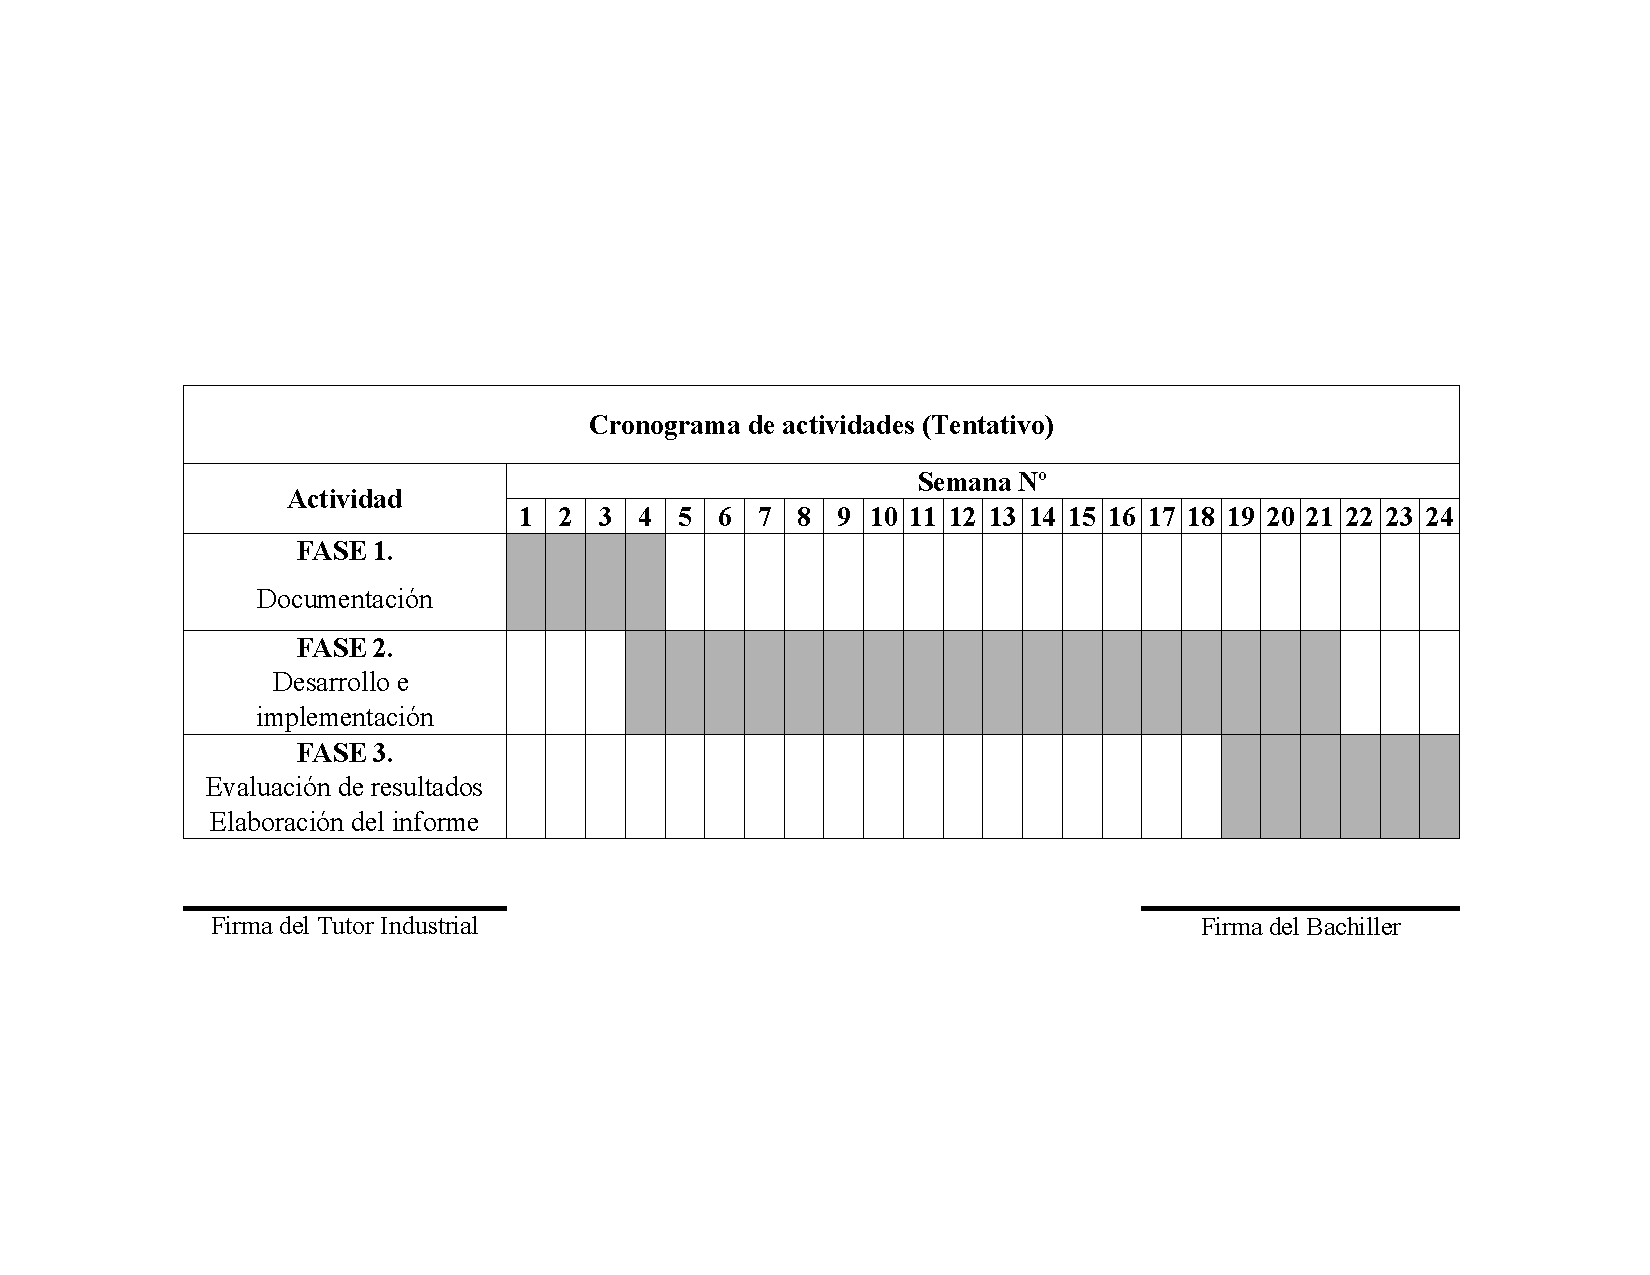
\includepdf[landscape]{DiagramadeGantt}
\end{document}
